\documentclass[aspectratio=169]{beamer}

% ---------- THEME & LOOK ----------
\usetheme{Madrid}
\usecolortheme{seahorse}
\usefonttheme{professionalfonts}
\setbeamertemplate{navigation symbols}{}
\setbeamercovered{transparent}
\setbeamertemplate{itemize items}[circle]
\setbeamertemplate{enumerate items}[default]
\setlength{\parskip}{0.25em}

% ---------- COLORS ----------
\usepackage{xcolor}
\definecolor{accent}{RGB}{0,92,184}
\definecolor{soft}{RGB}{233,244,255}
\setbeamercolor{structure}{fg=accent}
\setbeamercolor{title}{fg=white,bg=accent}
\setbeamercolor{frametitle}{fg=accent}
\setbeamercolor{block title}{bg=accent!10,fg=accent}
\setbeamercolor{block body}{bg=soft}

% ---------- PACKAGES ----------
\usepackage{booktabs}
\usepackage{amsmath, amssymb}
\usepackage{array}
\usepackage{hyperref}
\hypersetup{colorlinks=true,linkcolor=accent,urlcolor=accent}

% ---------- PLACEHOLDER BOX (compile-safe; no images required) ----------
\newcommand{\placeholderbox}[2][0.82\linewidth]{%
  \begin{center}
    \fbox{\begin{minipage}[c][0.46\textheight][c]{#1}
      \centering \vspace{0.25em}
      \textbf{#2}\\[0.6em]
      \emph{Insert figure/diagram here later.}
    \end{minipage}}
  \end{center}
}

% ---------- TITLE ----------
\title{\textbf{Compensating Wage Differentials \vspace{.5cm}\\  }}
\subtitle{ {\large ECON 300 - Labour Economics}}
%\institute{UNBC}
\author{Muhebullah Karimzada}

\date{Winter 2026}


\begin{document}

% ============================================================
% TITLE
% ============================================================
\begin{frame}[plain]
  \titlepage
\end{frame}

% ============================================================
\section{Orientation}
% ============================================================

\begin{frame}{Learning Objectives}
\transfade
\begin{itemize}[<+->]
  \item Explain how wages reflect job attributes: working conditions, shift work, pensions, health benefits, and risk.
  \item Identify when market-determined workplace risk can be optimal and when it will not be.
  \item Evaluate how safety regulations can raise or lower overall welfare.
    \item Understand “no free lunch”: workers often \textbf{pay} for desirable perks via lower wages.
  \item Use compensating wage premia for risk to infer the \emph{value of a statistical life} (VSL).
\end{itemize}
\end{frame}



\begin{frame}{Main Questions}
\transfade
\begin{itemize}[<+->]
  \item What determines relative pay rates across jobs?
  \item Can equally skilled workers earn different wages in the neoclassical model?
  \item Do safety regulations make workers better or worse off?
  \item Are workers fully compensated for unpleasant or risky tasks?
\end{itemize}
\end{frame}

% ============================================================
\section{Purposes of Wages and Wage Structures}
% ============================================================

\begin{frame}{Purposes of Wages and Wage Structures}
\transfade
\begin{block}{Wage Structure}
A hierarchy/grid of wage levels; a set of \textbf{premiums} linked to worker or job attributes.
\end{block}
\begin{itemize}[<+->]
  \item \textbf{Wage–productivity link:} Pay must cover marginal productivity (in competitive settings).
  \item \textbf{Social role:} Wages also signal status, fairness, and help align incentives.
\end{itemize}
\end{frame}

% ============================================================
\section{Theory of Compensating Wages}
% ============================================================

\begin{frame}{Smith’s Compensating Differentials: What Gets Priced?}
\transfade
\begin{itemize}[<+->]
  \item Agreeableness/disagreeableness of tasks
  \item Training cost and difficulty
  \item Turnover/retention aspects
  \item Responsibility, power, trust
  \item Probability of success
  \item \textbf{Safety and risk}
\end{itemize}
\end{frame}

\begin{frame}{Isoprofit Schedules (Firms’ Side)}
\transfade
\begin{itemize}[<+->]
  \item Combinations of \textbf{wage} and \textbf{safety} that yield the same profit.
  \item Diminishing MRT between wages and safety; lower curves \(\Rightarrow\) higher profits.
\end{itemize}
\end{frame}

\begin{frame}{Figure 8.1: Employer’s Isoprofit Schedules and Offer Curve }
\centering
\vspace{3.5em}

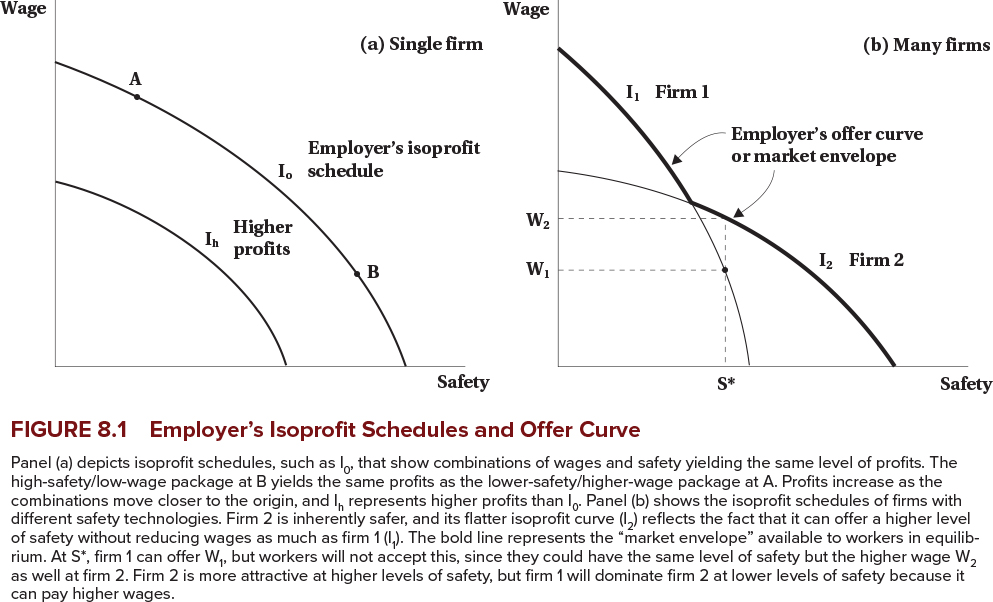
\includegraphics[width=0.99\linewidth]{ben54842_0801}
\end{frame}

\begin{frame}{Different Safety Technologies Across Firms}
\transfade
\begin{itemize}[<+->]
  \item Firms differ in the \textbf{cost} of providing safety.
  \item For the same profit, different firms have different isoprofit curves.
\end{itemize}
\end{frame}

\begin{frame}{Worker Preferences and Indifference Curves}
\transfade
\begin{itemize}[<+->]
  \item Iso-utility curves over \textbf{safety} and \textbf{wage}.
  \item More risk-averse workers need higher premia to accept risk.
\end{itemize}
\end{frame}

\begin{frame}{Figure 8.2: Worker Indifference Curves }
\centering
\vspace{5em}

\includegraphics[width=0.9\linewidth]{ben54842_0802}
\end{frame}

\begin{frame}{Equilibrium with One Firm and One Worker}
\transfade
\begin{itemize}[<+->]
  \item \textbf{Tangency} of iso-utility and isoprofit \(\Rightarrow\) optimal wage–safety bundle.
  \item Trades off wage for safety based on preferences and technology.
\end{itemize}
\end{frame}

\begin{frame}{Many Firms, Many Workers (Sorting)}
\transfade
\begin{itemize}[<+->]
  \item With competition, workers \textbf{sort} into jobs by risk preferences; firms sort by safety technology.
  \item \textbf{Wage–safety locus:} Market envelope of equilibrium wage–safety combinations.
\end{itemize}
\end{frame}

\begin{frame}{Figure 8.3: Market Equilibrium }
\centering

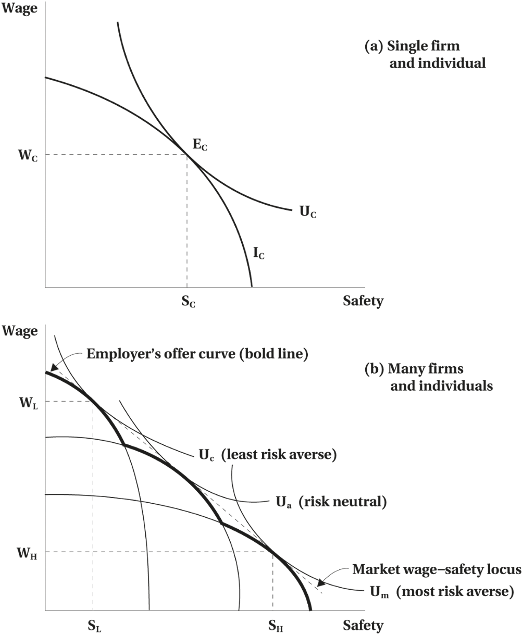
\includegraphics[width=0.79\linewidth]{ben54842_0803}
\end{frame}

\begin{frame}{Characteristics of the Wage–Safety Locus}
\transfade
\begin{itemize}[<+->]
  \item \textbf{Negative slope:} Lower safety requires compensating wages.
  \item \textbf{Curvature} depends on worker preferences and firm safety technology.
\end{itemize}
\end{frame}

% ============================================================
\section{Effect of Safety Regulation}
% ============================================================

\begin{frame}{Regulation in Competitive Markets}
\transfade
\begin{itemize}[<+->]
  \item Mandated higher safety can make one or both parties worse off if markets already internalize risk trade-offs.
  \item However, real-world frictions (info, externalities, imperfect competition) can justify regulation.
\end{itemize}
\end{frame}

\begin{frame}{Figure 8.4: Responses to a Safety Standard}
\centering
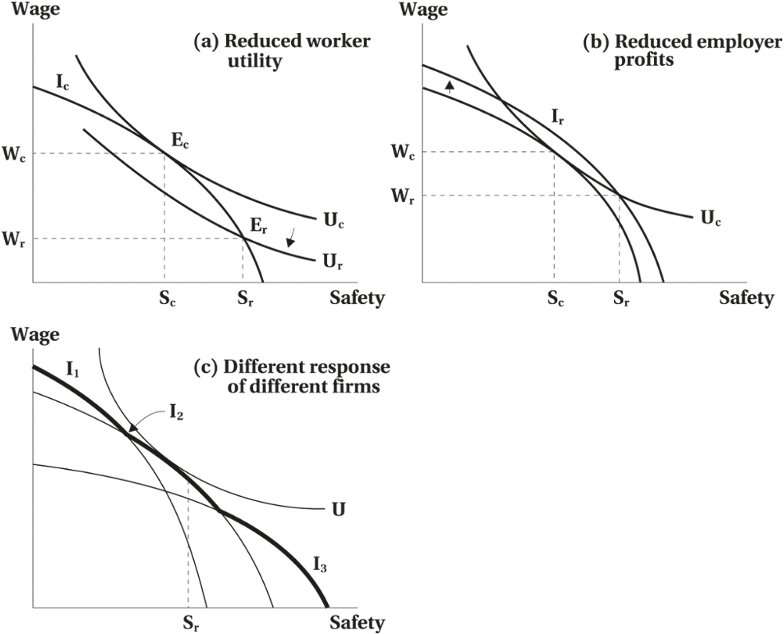
\includegraphics[width=0.59\linewidth]{ben54842_0804}
\end{frame}

\begin{frame}{Worked Example: Attracting Doctors to Rural Areas}
\transfade
\small
Two doctors can earn \$100{,}000 in a city.
\begin{itemize}[<+->]
  \item Dr.\ Brown’s city amenity value is \$90{,}000 \(\Rightarrow\) indifferent between \$100{,}000 (city) and \$190{,}000 (rural).
  \item Dr.\ Lewis’s amenity value is \$40{,}000 \(\Rightarrow\) indifferent between \$100{,}000 (city) and \$140{,}000 (rural).
  \item \textbf{Implication:} Rural premia must differ across workers to induce relocation; sorting yields higher rural pay.
\end{itemize}
\end{frame}

\begin{frame}{Location Decision Illustration }
\centering

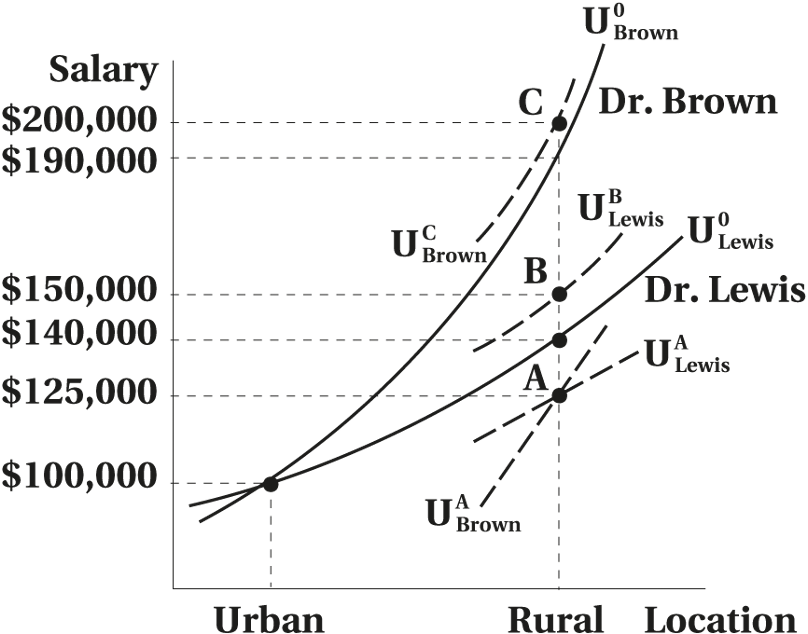
\includegraphics[width=0.6\linewidth]{ben54842_0801a}
\end{frame}

\begin{frame}{Imperfect Information}
\transfade
\begin{itemize}[<+->]
  \item If workers misperceive risk, mandated safety can raise their utility \emph{and} keep employers whole.
  \item Providing accurate information can move the market toward the optimal risk level.
\end{itemize}
\end{frame}

\begin{frame}{Figure 8.5: Effect of Imperfect Information }
\centering

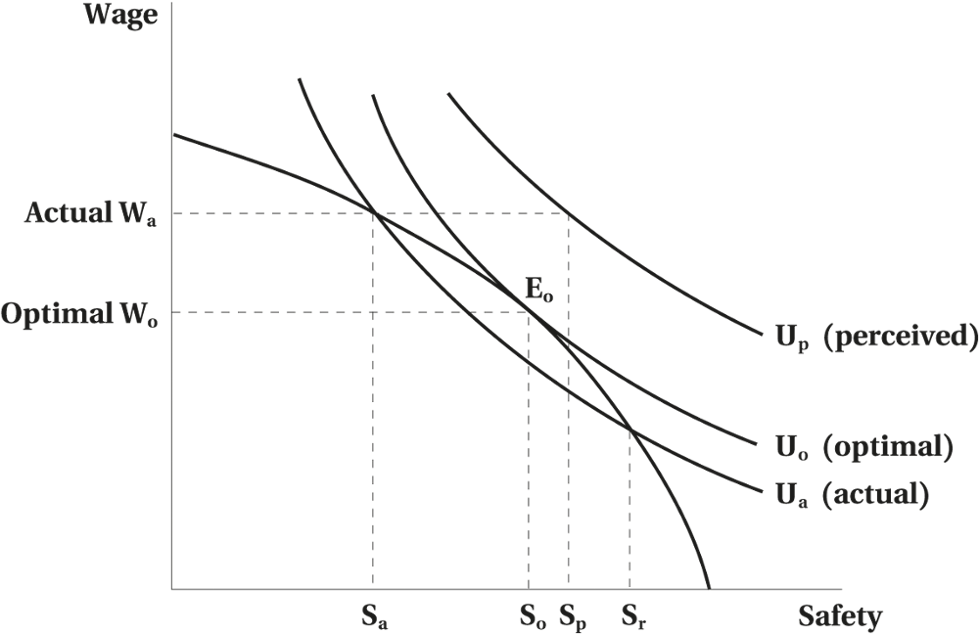
\includegraphics[width=0.69\linewidth]{ben54842_0805}
\end{frame}

\begin{frame}{Why Regulate?}
\transfade
\begin{itemize}[<+->]
  \item Information failures and non-competitive markets
  \item External costs of accidents not borne by workers/firms alone
  \item Social preferences for safety; behavioral biases (risk-as-feelings, present bias, “mental accounts,” wishful thinking)
\end{itemize}
\end{frame}

% ============================================================
\section{Empirical Evidence on Compensating Wages}
% ============================================================

\begin{frame}{Methodological Challenges}
\transfade
\begin{itemize}[<+->]
  \item Simultaneous equation bias (jobs \(\leftrightarrow\) wages)
  \item Errors-in-variables (risk mismeasurement)
  \item Omitted variables (unobserved ability/amenities)
  \item Sample selection (who takes risky jobs)
\end{itemize}
\end{frame}

\begin{frame}{Wage–Risk Trade-offs and Value of Life}
\transfade
\begin{itemize}[<+->]
  \item Risk premia \(\uparrow\) with severity of hazards.
  \item Coverage via workers’ compensation lowers required wage premia.
  \item Estimated wage–risk gradients \(\Rightarrow\) VSL measures.
\end{itemize}
\end{frame}

\begin{frame}{Desirable vs.\ Undesirable Job Characteristics}
\transfade
\begin{itemize}[<+->]
  \item Evidence of trade-offs: e.g., health insurance benefits vs.\ wages.
  \item Some amenities (e.g., flexible work) show clear wage offsets; others less so.
\end{itemize}
\end{frame}

\begin{frame}{Employment Security}
\transfade
\begin{itemize}[<+->]
  \item Compensating differentials for unemployment risk are theorized.
  \item Public UI provision complicates identification of pure wage premia.
\end{itemize}
\end{frame}

\begin{frame}{Family-Friendly Work Practices}
\transfade
\begin{itemize}[<+->]
  \item Substantial pay–amenity trade-offs for many family-friendly practices.
  \item Limited or no trade-off for childcare support or working from home in some contexts.
  \item Mandated maternity leave associated with wage adjustments for affected groups.
\end{itemize}
\end{frame}

\begin{frame}{Policy Implications}
\transfade
\begin{itemize}[<+->]
  \item Uniform standards can unintentionally reduce welfare if heterogeneity is large.
  \item Beware “double compensation” when benefits and insurance both cover the same risk.
  \item Compensating differentials help explain persistent wage structures across jobs, industries, and regions.
\end{itemize}
\end{frame}

% ============================================================
\section{Chapter Summary}
% ============================================================

\begin{frame}{Summary}
\transfade
\begin{itemize}[<+->]
  \item Compensating differentials price job attributes; workers trade wages for safety/amenities.
  \item Market equilibrium along a wage–safety locus reflects preferences and technologies.
  \item Regulation can help under information failures, externalities, or imperfect competition.
  \item Empirics require care: identification, measurement, and selection challenges.
\end{itemize}
\end{frame}

% ============================================================
\begin{frame}
\centering
\Huge{\textbf{Thank You!}} \\

\end{frame}

\end{document}
